\chapter{Background and related Work}
\label{ch:background}
This chapter covers the background and theoretical foundation of this work. A theoretical example case is used to ilustrate the expected performance behaviour of the WebCrowd platform. \autoref{sec:background:related_work} presents related works to describes the state of research and development in the field of volunteer computing and edge computing with WebAssembly.

\section{Distributed Computing \& Volunteer Computing}
Distributed computing describes a architecture where many autonomous computing elements collaborate as a unified system to solve complex computational problems through coordinated sharing of resources. A distributed computing system typically consists of multiple independent nodes, each possessing local memory and computational resources, interconnected through a network infrastructure that facilitates communication and synchronization between processes. This concept is particularly suitable to compute parallelizable workloads.

Volunteer Computing is a sub category of distributed computing that focuses on puplic support. Participants share their computer processing power to support a collective interest. The idea of volunteer computing already emerged in 1996 \cite{relatedwork:boinc1} and \citeauthor{background:vcname} later characterized the term \emph{volunteer computing} \cite{background:vcname}. The first large-scale scientific projects SETI@home and Folding@Home where launched in 1999 \cite{relatedwork:boinc1,relatedwork:seti}. These pioneering projects are since than demonstrating the success and popularity of volunteer computing.

Since the total amount of edge devices like laptops, smartphones, tablets and desktop computers continues to increase (TODO: QUELLE) there is a big pool of devices that can be used for volunteer computing. A study in 2014 has estimated that about 2 Billion computers are aktively in use worldwide \cite{intro:computersAmount,relatedwork:boinc1}. However, many of these resources often remain idle or underutilized during regular operation (TODO: QUELLE). While these untapped resources may seem insignificant individually, they collectively represent substantial potential due to their total number. These available resources located in office buildings, universities or public spaces can participate in volunteer computing projects to share their unused computational capabilities.

Furthermore, a study of 2011 revealed significant potential acceptance of volunteer computing in society, with 37\% of respondents indicating they were either \emph{"somewhat likely"} or \emph{"very likely"} to participate in volunteer computing projects \cite{intro:volunteerStudy}. However, the study also identified privacy and security concerns as primary factors that negatively influence willingness to volunteer in such projects \cite{intro:volunteerStudy}.

\section{Theory}
\label{sec:background:theory}
This following section displays the mathematical and theoretical background of the developed volunteer computing network. The objective is to identify the constraints that must be satisfied to ensure that the use of a volunteer computing network offers advantages over regular local computing on a single device.

The primary constraint is that the program code, which is distributed across multiple devices, must be capable of parallel execution. This allows all participating devices to  each compute a portion of the overall workload simultaneously. In this context, a parallelizable problem, as defined in this work, is characterized by the following properties:
\begin{itemize}
  \item The problem can be divided into multiple tasks.
  \item Each task executes the same program code.
  \item Each task can receive specific input parameters to process a distinct part of the problem.
  \item Each task operates independently, with no need for communication between tasks and no dependencies to other sequentially preceding tasks.
\end{itemize}
The total estimated execution time of a problem that is divided into \emph{T} equally sized tasks which are executed sequentially is denoted as $t_{ExSeq}$. It is assumed that, on average, each task requires a computing time of $t_{C}$ when executed. Consequently, the total computation time for the sequential execution of a problem on a single device is expressed as:
\begin{equation}
  t_{ExSeq} = T \cdot t_{C}
  \label{equ:single}
\end{equation}
When \emph{T} equal tasks are distributed over \emph{N} independent nodes, the total computation time is expected to be proportionally reduced, hece the workload is being parallelized. This reducing factor \emph{I} represents the amount of iterations needed to distribute all tasks \emph{T} over \emph{N} nodes and is described by the fraction of \emph{T} devided by \emph{N}. Since \emph{T} and \emph{N} are part of the natural numbers $\mathbb{N}$ and a single task can not be divided into smaller chunks, \emph{I} is also part of the natural numbers $\mathbb{N}$. To esure that the result of the devision is always a natural number the gaussian ceiling function is applied here. Hence, \emph{I} is given by: 
\begin{equation}
  I = \bigg\lceil\frac{T}{N}\bigg\rceil
  \label{equ:frac}
\end{equation}
When a problem is distributed across \emph{N} nodes over a wireless connection, the network latency must be taken into account in the computation of the total execution time $t_{ExDist}$. The latency, denoted as $t_{L}$, consists of the time required to send input arguments to a single device and the time needed to receive the result from a single task. It is assumed that the program code necessary to execute a task is loaded on all devices in advance, and therefore, the initial overhead of this process is excluded from the calculation. Additionally, it is assumed that the computation time $t_{C}$ of a task is equally long across all \emph{N} nodes. Thus, the total execution time $t_{ExDist}$ for a parallelizable problem distributed across \emph{N} nodes can be expressed as: 
\begin{alignat}{4}
  t_{ExDist} &= I \cdot (t_{C} + t_{L}) \nonumber \\
  t_{ExDist} &= \bigg\lceil\frac{T}{N}\bigg\rceil \cdot (t_{C} + t_{L})
  \label{equ:multiple}
\end{alignat}
The objective is to reduce the total computation time of a problem by distributing the workload across multiple nodes in parallel. This means that the execution time on a single device $t_{ExSeq}$, as described by \eqref{equ:single}, must be longer than the execution time on multiple devices $t_{ExDist}$, as described by \eqref{equ:multiple}. This leads to following inequality expression:
\begin{alignat}{4}
  t_{ExSeq} &> t_{ExDist} \nonumber \\
  T \cdot t_{C} &> \bigg\lceil\frac{T}{N}\bigg\rceil \cdot (t_{C} + t_{L})
  \label{equ:compare}
\end{alignat}
In order to transform this inequality, the term needs to be simplified by substituting the gaussian bracket. The value of \emph{I} can be overestimated by the following term:
\begin{equation}
  I = \bigg\lceil\frac{T}{N}\bigg\rceil \quad < \quad \frac{T}{N} + 1
  \label{equ:frac2}
\end{equation}
This overestimate is used to substitude the value of \emph{I} in function \ref{equ:multiple} to create following inequality expression:
\begin{equation}
  T \cdot t_{C} > \bigg(\frac{T}{N} + 1\bigg) \cdot (t_{C} + t_{L})
  \label{equ:substitution}
\end{equation}
This allows following transformation of the inequality of \ref{equ:substitution}:
\begin{alignat}{4}
  T \cdot t_{C} &> \bigg(\frac{T}{N} + 1\bigg) \cdot (t_{C} + t_{L}) \nonumber \\
  T \cdot t_{C} &> \bigg(\frac{T + N}{N}\bigg) \cdot (t_{C} + t_{L}) \nonumber \\
  \frac{T \cdot N \cdot t_{C}}{T + N} &> t_{C} + t_{L} \nonumber \\
  \frac{T \cdot N \cdot t_{C}}{T + N} - t_{C} &> t_{L} \nonumber \\
  t_{C} \cdot \bigg(\frac{T \cdot N}{T + N} - 1\bigg) &> t_{L}
  \label{equ:transformation}
\end{alignat}
The last expression through the transformation in \eqref{equ:transformation} results in the constrain, that distributing a parallelizable problem across multiple nodes is only beneficial if the latency $t_{L}$ is shorter than the computation time of a single task multiplied by the factor $(\frac{T \cdot N}{T + N} - 1)$.

Additionally the expression from \eqref{equ:frac} can be used to determine the optimal amount of nodes \emph{N} for a problem divided in \emph{T} equally sized tasks. The number of iterations \emph{I} reaches its minimum of $1$ if \emph{N} and \emph{T} are equally sized. This outcome is intuitive, as in this ideal scenario each node is rersponsible for a single task and therefore all tasks \emph{T} are executed simultaneously. Furthermore can be concluded from \eqref{equ:frac} that the amount of nodes should ideally be a divisor of \emph{T} to ensure a efficient utilization of all nodes. However, in practice, it should be considered to include additional backup devices in the network to account for potential failures or disruptions.

\subsection{Theoretical Case}
To illustrate the performance gain achieved by a volunteer computing network, both expressions \eqref{equ:single} and \eqref{equ:multiple} are plotted in \autoref{fig:background:theoryplot}. To calculate these graphs, an Internet latency of 32 ms \cite{backend:latency} was assumed. This value is the \ac{IQI} estimated round trip time within Europe \cite{backend:latency}. The average computation time $t_{C}$ for a single task was assumed to be 34.97 s, based on the measured average run time of the source code in \autoref{app:code:mandelbrot1} on the system specified in \autoref{app:system:mymachine}. This measurment was repeated with a WebAssembly binary, generated with the source code in \autoref{app:code:mandelbrot2}. The average execution time of the WebAssembly binary in a browser environment (Mozilla Firefox 132.0 \cite{background:firefox}) on the system specified in \autoref{app:system:mymachine} was measured at 71.17 seconds, being about 2.04 times slower. 
\newline
\begin{addmargin}[25pt]{25pt}
  This is an unexpected difference in computation duration between native and WebAssembly code execution, since WebAssembly is promissed to perform at near-native speed \cite{methodology:wasm}. \citeauthor{background:not-so-fast} stated in their work that WebAssembly shows a significantly worse performance compared to native code, with an average performance gap of 45\% (Firefox) to 55\% (Chrome) and peak slowdowns of 2.08x (Firefox) and 2.5x (Chrome) across measured SPEC CPU benchmarks \cite{background:not-so-fast}. This matches the unexpected slowdown of 2.04 measured in the previously mentioned experiment. \citeauthor{background:not-so-fast} identified the following performance issues to be the root cause of the experienced performance gap when using WebAssembly \cite{background:not-so-fast}:
  \begin{enumerate}
    \item \emph{Increased Register Pressure}
    \item \emph{Extra Branch Instructions}
    \item \emph{Increased Code Size}
  \end{enumerate}
\end{addmargin}
In the modeling of this theoretical case is an additional initial offset time considered, which estimates the time needed to establish the volunteer computing network. In this process, each node must download all necessary files in advance to be able to execute the workload. Since this setup occurs in parallel across all nodes, the offset matches the time required for the setup of a single node. This offset value is calculated using the \ac{IQI} estimated download speed in Europe of 29 Mbps \cite{backend:latency}. The size of the compiled WebAssembly binary file from the source code in \autoref{app:code:mandelbrot2} is 21.6 Mb (2.7 MB), and the coresponding \emph{wasm\_exec.js} JavaScript file to setup the WebAssembly environment is 0.13 Mb (16.7 KB), resulting in a total file size of 21.73 Mb. The time required to download both files to a single node can be estimated using the following expression:
\begin{equation}
  DownloadTime = Latency + \frac{Filesize}{Bandwith} 
  \label{equ:offset}
\end{equation}
Since the bandwidth is given in megabits per second, while the latency is provided in milliseconds, the latency value needs to be converted to seconds. Using the calculation in \ref{equ:offset}, the additional offset that is required to set up the platform, in this theoretical case, is estimated to be at least 0.78 s.

\begin{figure}[htbp]
  \myfloatalign
  \subfloat[Variable amount of nodes N]{
     \label{fig:background:theoryA}
     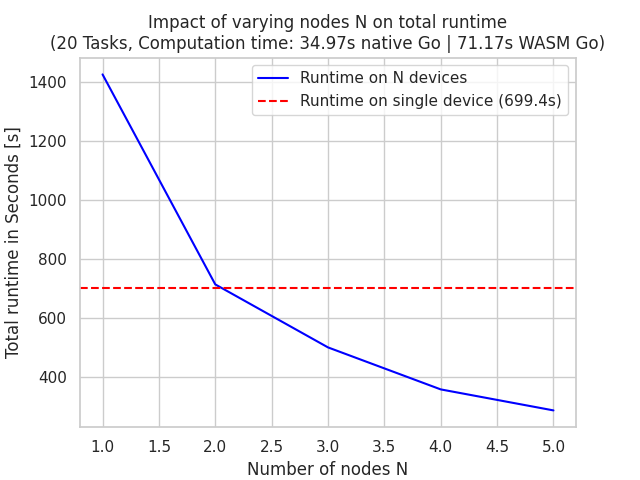
\includegraphics[width=.48\linewidth]{gfx/figures/Theory_A.png}
   } 
   \subfloat[Variable amount of tasks T]{
     \label{fig:background:theoryB}
     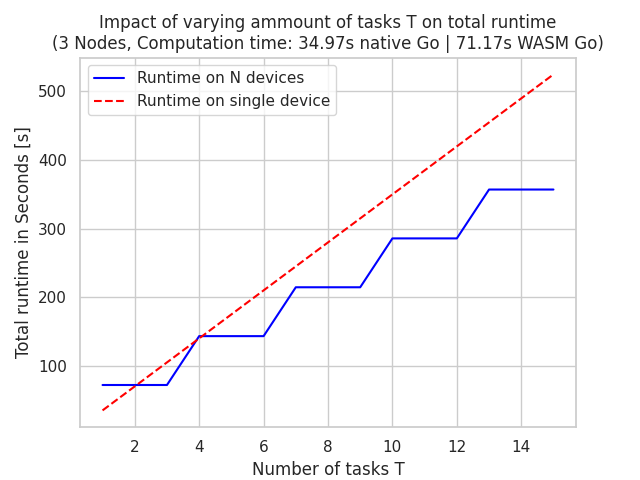
\includegraphics[width=.48\linewidth]{gfx/figures/Theory_B.png}
   }
   \caption{Visualizing the Total Computation Time for an Estimated Example Case}
   \label{fig:background:theoryplot}
\end{figure}
~\\
The graph in \autoref{fig:background:theoryA} represents the total runtime, on the y-axis in seconds, as a function of the number of nodes $N$ in the network, on the x-axis. The red dotted line displays the performance of a single machine $t_{ExSeq}$, while the blue line illustrates the performance of the volunteer computing network $t_{ExDist}$. The total number of all tasks $T$ is set to 20. This plot reveals that the volunteer network achieves a faster total computation time than a single device, if three or more nodes are availabile in the network. The total runtime $t_{ExDist}$ is already by 30\% faster than $t_{ExSeq}$ when the workload is distributed to three nodes.

The other graph in \autoref{fig:background:theoryB} displays the total runtime on the y-axis in seconds as a function of the number of tasks $T$ on the x-axis. The red dotted line represents again $t_{ExSeq}$ of a single device and the blue line $t_{ExDist}$ of the volunteer computing network. The number of nodes $N$ is set to three. This plot demonstrates that the volunteer network achieves faster total computation time than a single device when the workload $T$ consists of more than two tasks. The performance gain grows exponentially as the number of tasks increases. Furthermore, it can be concluded that the total computation time $t_{ExDist}$ of the volunteer network only increases when the number of tasks $T$ and the number of nodes $N$ have no common divisor. However, it is crucial to note that the network will have a longer computation time in every scenario with only one task, as a single task cannot be executed in parallel.

Both plots show, that the total computation time $t_{ExDist}$ is already almost even to the threshold value of $t_{ExSeq}$ if the volunteer network has two participating nodes and faster if there are three or more nodes. This holds true even if the computation time $t_{C}$ of a single task is twice as fast on a native system as measured in the browser environment. This proves that the approach of distributing the workload has a performance gain in this theoretical example, if multiple nodes participate in the volunteer computing network. 

However it needs to be considdered, that if there is only one or two node in the network this approach will already be slower in this example due to the initial offset time, the additional network latency and the higher computation time for each individual task.

\section{Related Work}
\label{sec:background:related_work}
The idea of volunteer computing has been established for a long time. The earliest concept of volunteer computing started already back in 1996 \cite{relatedwork:boinc1}. This section introduces relevant projects in this field, which have been used in the past or are currently in active use and maintenance.

\subsection{BOINC}
\label{subsec:background:related_work:boinc}
\ac{BOINC} is an open-source middleware system for volunteer computing, which utilizes consumer devices for scientific computing. It addresses key challenges in distributed computing, such as dealing with untrusted, unreliable, and heterogeneous computing resources, validating results from potentially malicious hosts, and supporting diverse applications and computing environments. \cite{relatedwork:boinc1}

The BOINC architecture consists of server components, including a database and job scheduler, and client software comprising a core client, GUI, and screensaver. Communication between clients and servers is facilitated through HTTP-based RPCs. BOINC employs replication-based validation and adaptive replication to ensure result integrity while minimizing overhead. The system also implements sophisticated scheduling policies both on the client and server sides to optimize resource allocation and job dispatch. \cite{relatedwork:boinc1}

BOINC has been successful in supporting numerous scientific projects and providing substantial computing power. \cite{relatedwork:boinc1}

\subsection{SETI@home}
\label{subsec:background:related_work:seti}
\ac{SETI} at home (\ac{SETI}@home) represents a pioneering project in the field of distributed and volunteer computing. It utilises the resources of volunteer computers worldwide to analyze radio telescope data in search of extraterrestrial intelligence. Data from the Arecibo radio telescope is divided into smaller chunks which are distributed to volunteer computers for processing. The system is designed to identify several types of patterns in radio signals that could indicate an artificial origin. These anormalies are spikes, Gaussians, pulsed signals, and triplets in the collected radio data. \cite{relatedwork:seti}

Back in the year 2002, \ac{SETI}@home had engaged over 3.8 million participants across 226 countries, achieving an average computing power of 27.36 teraFLOPS \cite{relatedwork:seti}.

\ac{SETI}@home demonstrated the viability of large-scale public-resource computing and identified key factors that make tasks suitable for this approach:
\begin{itemize}
  \item High computing-to-data ratio
  \item Independent parallelism
  \item Error tolerance
  \item Ability to attract public interest
\end{itemize}
The success of \ac{SETI}@home not only advanced scientific research but also increased public awareness and involvement in scientific participation. This project laid therefore the groundwork for future volunteer computing projects and frameworks. \cite{relatedwork:seti}

\subsection{XtremWeb}
\label{subsec:background:related_work:xtremweb}
XtremWeb is an experimental Global Computing platform designed to harness idle computing resources connected to the Internet for high-throughput computing. The system aims to provide a platform for experimenting with Global Computing capabilities and addressing issues such as scalability, heterogeneity, availability, fault tolerance, security, and usability in massively distributed computing environments. \cite{relatedwork:xtremweb}

The architecture of XtremWeb consists of three main components:
\begin{enumerate}
  \item Workers: These are volunteer PCs that execute tasks. They are implemented primarily in Java for portability, with native code used for OS-specific functions. Workers monitor resource availability based on user-defined policies and support multiple platforms, including Linux and Windows.
  \item Servers: These manage tasks and applications. The server design is modular, with components for application pool, job pool, accounting, and scheduling. Servers can be clustered for increased throughput and support specialization for tasks such as dedicated result collection.
  \item Clients: These submit tasks to the system.
\end{enumerate}
XtremWeb employs a two-part scheduling system:
\begin{enumerate}
  \item Dispatcher: Selects tasks from the pool based on application priorities.
  \item Scheduler: Assigns tasks to workers.
\end{enumerate}
The default scheduling policy of XtremWeb is FIFO and XtremWeb implements a timeout to enable rescheduling of aborted tasks \cite{relatedwork:xtremweb}.

Furthermore XtremWeb implements a worker-initiated communication protocol, which facilitates easier deployment through firewalls. This protocol consists of the four main requests: \emph{hostRegister}, \emph{workRequest}, \emph{workAlive}, and \emph{workResult}. \cite{relatedwork:xtremweb}

XtremWeb has been successfully applied to various projects in the past. Thes include the Pierre Auger Observatory for studying high-energy cosmic rays. In this application, XtremWeb was used to run the \ac{AIRES} program by partitioning large simulations into smaller subtasks. \cite{relatedwork:xtremweb}

In summary, XtremWeb provides a flexible and robust platform for experimenting with Global Computing concepts. Its approach and concept has some similarities to WebCrowd. The original XtremWeb project seems to be not maintained since its development in the early 2000s.

\subsection{EGEE}
\label{subsec:background:related_work:egee}
Initiated on April 1, 2004, \ac{EGEE} was a two-year project within a planned four-year program, involving 71 partners from Europe, Russia, and the United States \cite{relatedwork:egee}. The project's primary objectives were to establish a seamless European grid infrastructure for scientific research, provide production-level grid services, and re-engineer grid middleware for enhanced robustness and scalability \cite{relatedwork:egee}.

The infrastructure of \ac{EGEE} was built upon the EU Research Network GEANT, leveraging expertise from previous initiatives such as EU DataGrid, UK e-Science, INFN Grid, Nordugrid, and US Trillium. The project aimed to expand its computational capabilities from an initial 3000 CPUs at 10 sites to 10000 CPUs across 50 sites by the end of 2005 \cite{relatedwork:egee}.

\ac{EGEE} focused on two primary pilot applications: 
\begin{itemize}
  \item The \ac{LCG} for high-energy physics data analysis.
  \item Biomedical Grids addressing challenges in genomic database mining and medical database indexing
\end{itemize}
The project focused on re-engineering existing middleware to address issues from first-generation implementations and ensure adherence to \ac{OGSA} standards. This approach aimed to enhance the reliability and scalability of the grid infrastructure \cite{relatedwork:egee}.

In conclusion, the \ac{EGEE} project represented a significant effort to transform grid computing from a research concept into a practical infrastructure to support "e-science" across Europe.

\subsection{WebAssembly for Edge Computing}
\label{subsec:background:related_work:wasmedgecomputing}
[WebAssembly for Edge Computing: Potential and Challenges] \cite{relatedwork:wasmedgecomputing}